\documentclass[11pt, a4paper, USenglish]{article} % change ``USenglish'' to ``norsk'' if applicable.

\usepackage{kyblab} % Contains all included packages. See kyblab.sty.
\addbibresource{bibliography.bib} % Makes the bibliography file available to biblatex.

\begin{document}

% Titlepage
\title{Boat lab}
\author{Group 06\\Student 478433\\Student 478455\\Student 478386}
\date{\today}
\begin{titlepage}
    \maketitle
    \begin{figure}
    \centering
    
\includegraphics[width=0.5\textwidth]{figures/itk_ntnu}\\
    Department of Engineering Cybernetics
    \end{figure}
    \thispagestyle{empty}
\end{titlepage}

% TOC
\newpage
\tableofcontents
\thispagestyle{empty} % Avoid page numbering on the table of contents.

% Main content
\newpage
\setcounter{page}{1}
\section{Introduction}\label{sec:intro}
In this lab we were assigned multiple problems associated with control of a simulated ship. \\
The ship is simulated in MATLAB and Simulink. Control of the ship is done through MATLAB scripts. \\
We were assigned different problems raging from identifying the boat parameters, and identifying how the ship oscillates by creating a wave spectrum model. We made a PD controller for the ship and did an analisys of observability for the ship. In the end we created, and tuned, a Discrete Kalman Filter for estimating the states of the ship. \\
Labs like this are important in education of control engineers. Practical experience is essential to obtain a good understanding of a subject, and getting problems like this is therefore good. This lab grants practical experience on how to apply theory, tuning, and control systems in general.\\
This report is organized into multiple parts. The report follows the assignment manual closely, and answers the questions prompted. 

\section{Part 5.1 Assignment of the boat parameters}
\subsection{a}
Given the equations from \todo{Cite lab text}
\begin{subequations}
\begin{align}
    \dot{\xi} &= \psi_\omega\\
    \dot{\psi}_\omega &= -\omega^2_0 \xi_\omega - 2 \lambda \omega_0 \psi_\omega + K_\omega \omega_\omega\\
    \dot{\psi} &= r\\ \label{eq:start_psi}
    \dot{r} &= -\frac{1}{T} r + \frac{K}{T} (\delta-b)\\ \label{eq:start_r}
    \dot{b} &= \omega_b\\
    y &= \psi + \psi_\omega + v
\end{align}
\end{subequations}
We want to find the transfer function, $H(s)$, from $\delta$ to $\psi$. Taking the Laplace transform of \cref{eq:start_r} we get 
\begin{align*}
    \mathcal{L}\{\dot{r}\}(s) &= \mathcal{L}\{{-\frac{1}{T} r + \frac{K}{T}
    (\delta - b)}\}(s)\\
    s r&=-\frac{1}{T} r + \frac{K}{T}(\delta - b)\\
    r &= \frac{K}{T}(\delta-b) \frac{1}{s+\frac{1}{T}}
\end{align*}
Assuming there is no disturbances and substituting into  \cref{eq:start_psi} we then get
\begin{align}
    H(s) &= \frac{K}{s(Ts+1)}
\end{align}
\subsection{b}
Use the plots and show the derivation of the parameters K and T. Measured amplitude from scopes
$K = 0.1559$ and $T = 71.6865$
\begin{align*}
    \omega_1 &= 0.005\\
    \omega_2 &= 0.05\\
    K &= A_1\omega_1\sqrt{T^2\omega_1^2+1}\\
    T &= \sqrt{\frac{A_2^2\omega_2^2-A_1^2\omega_1^2}{A_1^2\omega_1^4-A_2^2\omega_2^4}}
\end{align*}
$$K = A_1\omega_1\sqrt{T^2\omega_1^2+1}$$

$$T = \sqrt{\frac{A_2^2\omega_2^2-A_1^2\omega_1^2}{A_1^2\omega_1^4-A_2^2\omega_2^4}}$$

\subsection{c}
Setting the measurement cursors at the peak without noise. 
Repeating the procedure we get $K = 0.3572$ and $T = 444.6904$
Is it possible to get good estimates?\\
We get decent estimates but is not that good when setting the frequency to 0.05. Maybe because the frequency of the waves is close to the frequency of the sine. 
\subsection{d}
Applied a step on both the full system model in Simulink and also on the transfer function using MATLAB. 
\begin{figure}
    \centering
    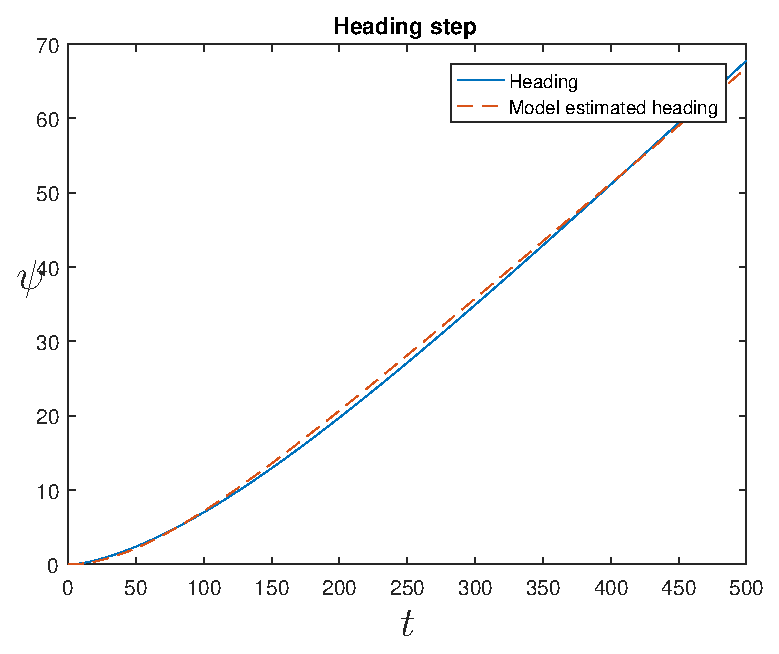
\includegraphics{figures/plots/p5p1d.eps}
    \caption{Caption\todo{}}
    \label{fig:my_label}
\end{figure}
\newcommand{\texMacro}[2]{\texttt{\textbackslash{#1}\{#2\}}}
\section{Part 5.2 Identification of the wave spectrum model}
\subsection{A, Estimating the Power Spectral Density function of $\psi_w$}
In this part we wish to estimate the Power Spectral Density- (PSD) function of how the waves impact the heading.  
Given data of how the waves influence the compass measurement, $\psi_w$ , we can find the PSD-function, named $S_{\psi_w}(\omega)$, using MATLAB. In \cref{PSD func matlab} we show how we calculated the PSD-function.\\
psi\_w is a data series of $\psi_w$, given in degrees. We scale it to radians.  
\begin{lstlisting}[caption={Calculating Power Spectral Density function},label={PSD func matlab}]
x = psi_w(2,:)*pi/180;
fs = 10;
[pxx,f] = pwelch(x,window, [], [], fs);
pxx=pxx./(2*pi);
f=f.*2*pi;
\end{lstlisting} 
Plotting (pxx, f), which is  $S_{\psi_w}$, we get \Cref{fig:Power Spectral density}. 
\begin{figure}
    \centering
    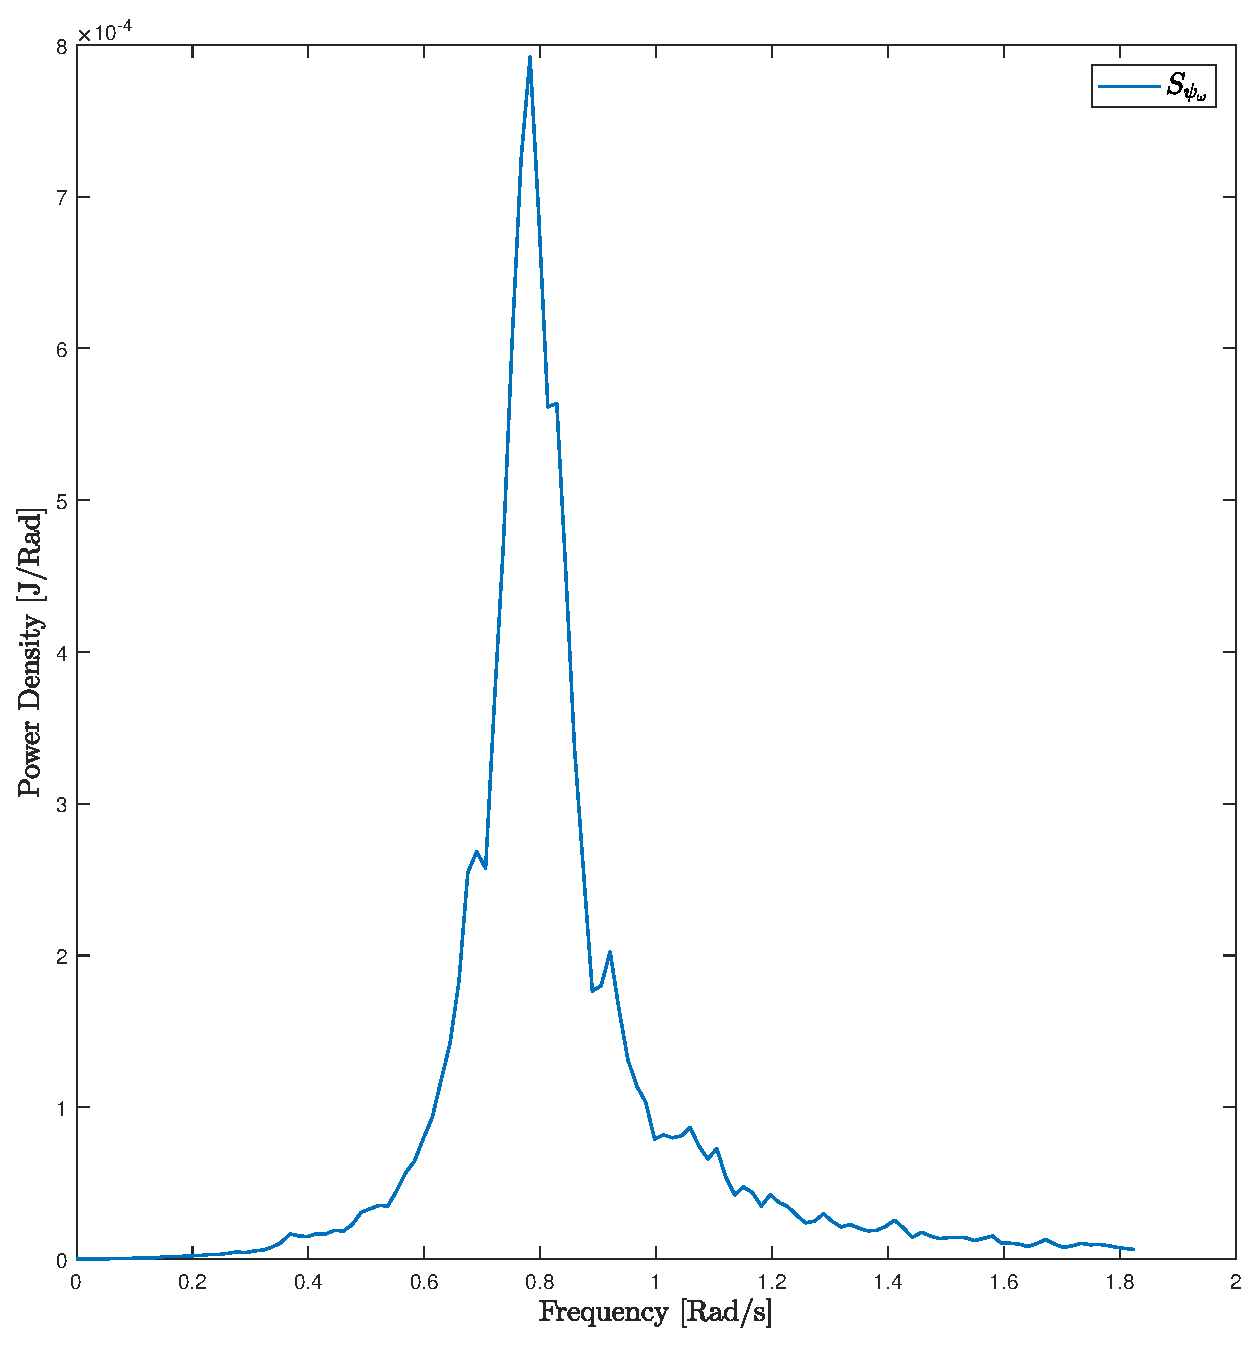
\includegraphics[width=1.00\textwidth]{figures/plots/P5p2a_PSD.eps}
    \caption{Power Spectral Density function for compass measurement}
    \label{fig:Power Spectral density}
\end{figure}


\subsection{B, Analytical expression for the Power Spectral Density}
Analytical expression for the transfer function of the wave response model

From \cite{assignment} we have the Namoto equations
\begin{align}
    \dot{\xi}_w &= \psi_w\label{eq:namoto1}\\
    \dot{\psi}_w &= -\omega_0^2\xi_w-w\lamda\omega_0\psi_w+K_{w}w_w\label{eq:namoto2}
\end{align}
Taking the Laplace transform of these and inserting \ref{eq:namoto1} into \ref{eq:namoto2} we get
\begin{align*}
    s\xi_w &= \psi_w\\
    s\psi_w &= -\omega_0^2\frac{\psi}{s} - w\lamda\omega_0\psi_w + K_{w}w_w\\
    (s^2+2\lambda\omega_0+\omega_0^2)\psi_w &= K_{w}w_w\\
    \frac{\psi_w}{w_w}(s) &= \frac{K_{w}s}{s^2+2\lamda\omega_0s+\omega_0^2}\\
    \hat{H}(j\omega) &= \frac{K_{w}s}{s^2+2\lamda\omega_0s+\omega_0^2}
\end{align*}
where $\hat{H}(j\omega)$ is the transfer function from $w_w$ to $\psi_w$.

Using the Wiener-Khinchin theorem \cite{Wiener-Kinchkin} we can find an analytical expression for the Power Spectral Density function for $\psi_w$. 
Using that $w_w$ is a zero mean white noise, we know that the Power Spectral Density function of $w_w$, called $P_{w_{w}}$, is 1. Thus we get that 
\begin{align*}
    P_{\psi_{w}} &= P_{w_w}\abs{\hat{H}(j\omega)}^2\\
    &= \hat{H}(-j\omega)\hat{H}(j\omega)\\
    &= \hat{H}(-j\omega)\hat{H}(j\omega)\\
    &= \hat{H}(-j\omega)\hat{H}(j\omega)\\
    &= \frac{(K_{w}j\omega)(-K_{w}j\omega)}{((j\omega)^2+2\lamda\omega_0j\omega+\omega_0^2)(-j\omega)^2-2\lamda\omega_0j\omega+\omega_0^2)}\\
    &= \frac{K_{w}^2\omega^2}{\omega^4+\omega^2\omega_0^2(4\lambda^2-2)+\omega_0^4}
\end{align*}


\subsection{C, Finding $\omega_0$ and $\sigma^2$}
Reading the values from \cref{fig:Power Spectral density} we get
\begin{align*}
    \omega_0 &= 0.07823\\
    \sigma &= 0.0281
\end{align*}
where $\omega_0$ is the frequency of peak intensity, and $\sigma^2$ is the peak frequency. 


\subsection{D, Identifying the dampening factor $\lambda$}
We want to identify the damping factor $\lambda$. Using 
$$K_w = 2\lambda\omega_0\sigma$$ 
we get 
$$P_{\psi_{w}} = \frac{4\lambda^2\omega_0^2\sigma^2\omega^2}{\omega^4+(4\lambda^2-2)\omega_0^2\omega^2+\omega_0^4}$$
By plotting $P_{\psi_w}$ versus $S_{\psi_w}$ and adjusting $\lambda$ until the plots overlay we find an estimate for $\lambda$. 

Thus we found that a decent value for lambda is $\lambda  = 0.09$. This value gave $P_{\psi_w}$ shown in \Cref{fig:PSD P vs S} plotted versus $S_{\psi_w}$.


\begin{figure}
    \centering
    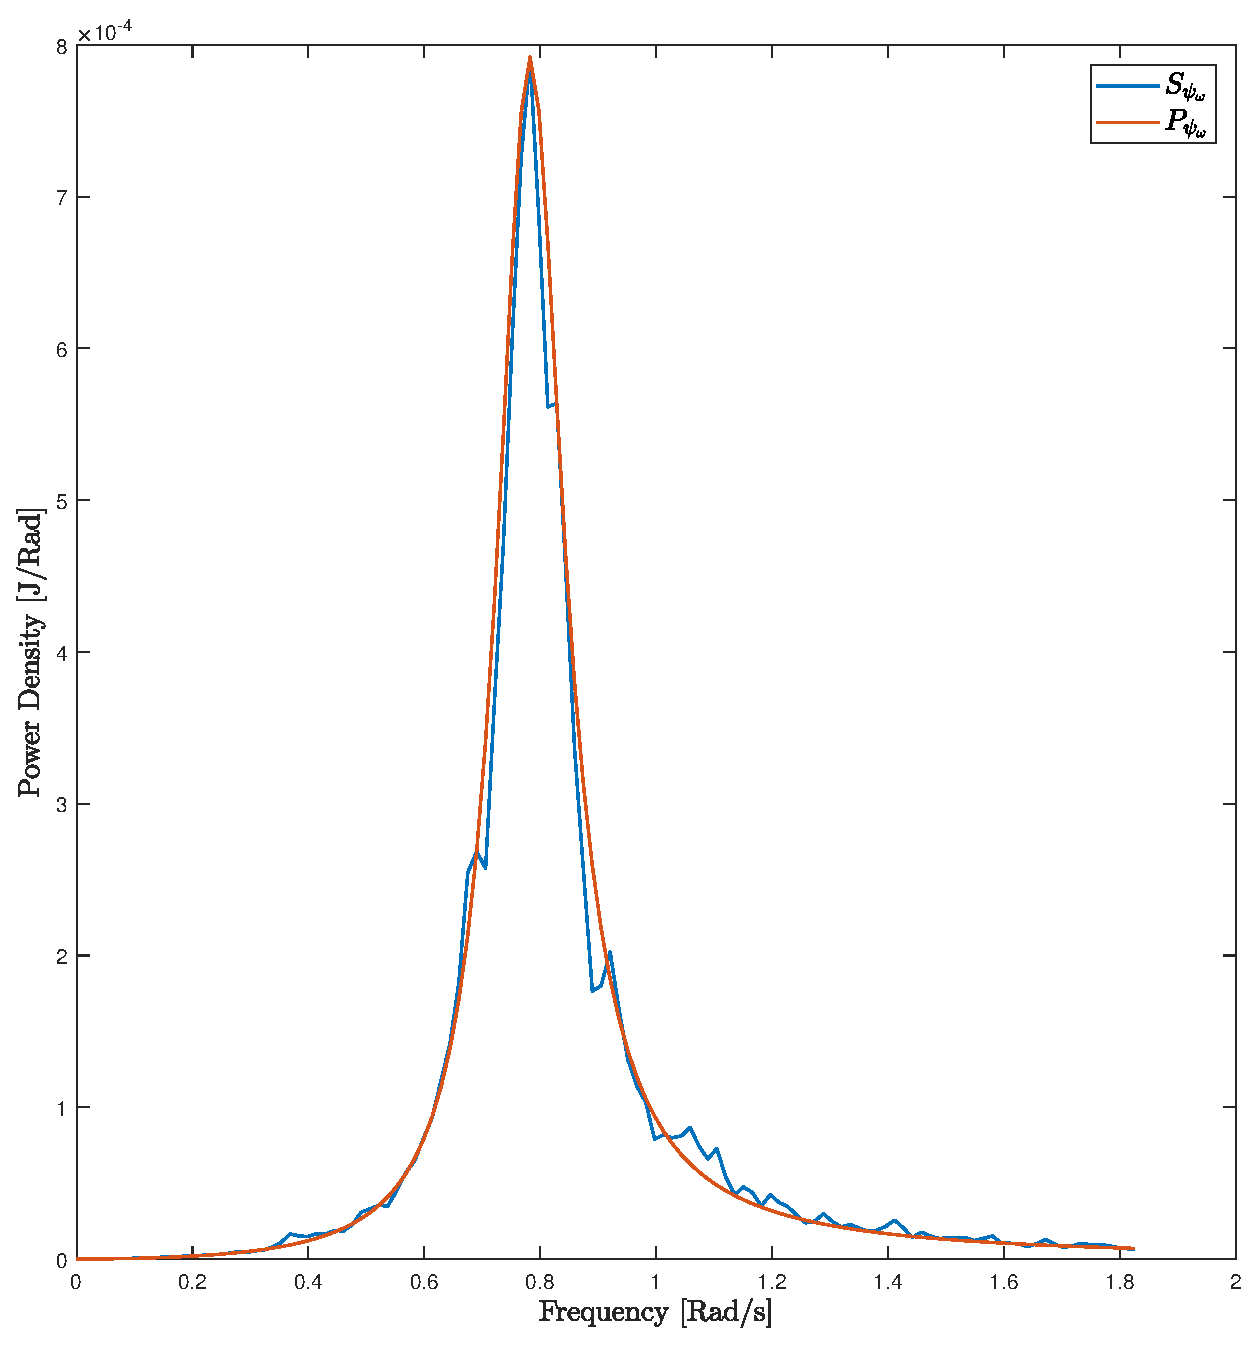
\includegraphics[width=1.00\textwidth]{figures/plots/P5p2d_lambda009rad.eps}
    \caption{$P_{\psi_w}$ plotted versus $S_{\psi_w}$, $\lambda$ = 0.09}
    \label{fig:PSD P vs S}
\end{figure}





\section{5.3 Control system design}
\subsection{A, Design of a PD controller}
A PD controller is given by the equation $H_{pd}(s) = K_{pd} \frac{1+T_ds}{1+T_fs}$. Using the transfer function \cref{eq:Transfer_function} from $\delta$ to $\psi$ without disturbances we define the open loop system as $H(s) \cdot H_{pd}(s)$. We chose $T_d=T$ to cancel the transfer function time constant. This reduces the order of the transfer function because the two terms cancels out. The open loop transfer function then becomes
\begin{align} \label{eq:transfer_function_open_loop}
    H(s) = \frac{K_{pd}K}{s(1+T_f s)}
\end{align} 
We wish to chose $K_{pd}$ such that the open loop system has $\omega_c = 0.10$ rad/s and a phase margin of $50 \deg$. 
\begin{align}
    \left| H(j\omega_c) \right| = 0 dB = 1 \notag \\
    \left| \frac{K_{pd}K}{j\omega_c(1+T_f j\omega_c)}\right| = 1 \notag \\
    \frac{K_{pd}K}{\omega_c \sqrt{1+T_f^2\omega_c^2}} = 1 \label{eq:length_tf}
\end{align}
The phase margin $\phi$ is defined as 
\begin{align}
    \phi = \angle H(j\omega_c) - (-180^\circ)
\end{align}
and by setting $\phi$ equal to $50^\circ$ we get
\begin{align}
    50^\circ = -90^\circ - \textrm{arctan}(T_f \omega_c)\notag \\
    T_f = \frac{\textrm{tan}(50^\circ-180^\circ+90^\circ}{\omega_c} = 8.4s
\end{align}
Now by inserting the obtained $T_f$ into \cref{eq:length_tf} we can solve for $K_{pd}$.
\begin{align}
    K_{pd} = \frac{\omega_c \sqrt{1+T_f^2\omega_c^2}}{K} = 0.839
\end{align}
\subsection{B, Implementation of PD controller and simulation without disturbances}
We implement the PD controller in Simulink as seen in \cref{fig:simulink_PD} and \cref{fig:simulink_total}. We set the reference $\psi_r = 30$ and simulate the system with only measurement noise, no disturbances. As we can see in \cref{fig:p3pb_rudder_heading} the ship reaches the reference pretty quickly and is able to hold keep the course stable. Thus the autopilot does its job quite satisfyingly. The rudder input is high in the start but as the system stabilizes it the size of the rudder input input moves to zero. It does however have some small vibrations due to the controller being sensitive to the measurement noise. The ship dynamics has a quite negative phase which results in either a slow controller or an oscillating response due to a small phase margin. A PD-controller lifts the phase of the full system and allows for higher $\omega_c$ resulting in quicker and more robust response than a P-controller. 
\begin{figure}
    \centering
    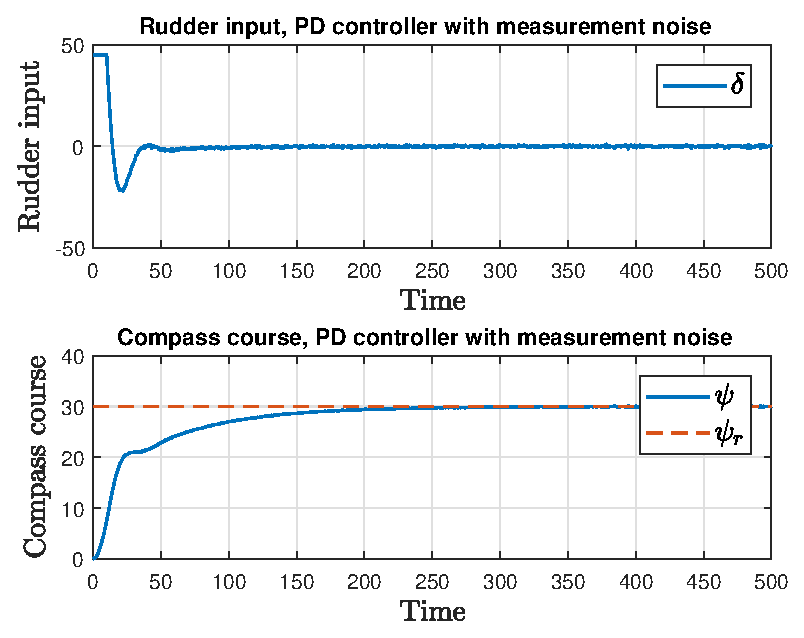
\includegraphics[width = 1.00\textwidth]{figures/plots/P5p3b_rudder_heading.eps}
    \caption{Rudder input and compass course response with a PD controller.}
    \label{fig:p3pb_rudder_heading}
\end{figure}
\subsection{C, Simulation with a current disturbance}
Now we simulate the system with current disturbance, measurement noise but no wave disturbance. As we can see in the \cref{fig:p3pc_rudder_heading}, the autopilot is no longer able to reach the reference of 30$\deg$. A stationary deviation of about 3.5$\deg$ is present. This is expected as we have no integral effect and the PD controller will only change the rudder input if the error changes. The rudder input never reaches zero but constantly tries to counteract the current disturbance.
\begin{figure}
    \centering
    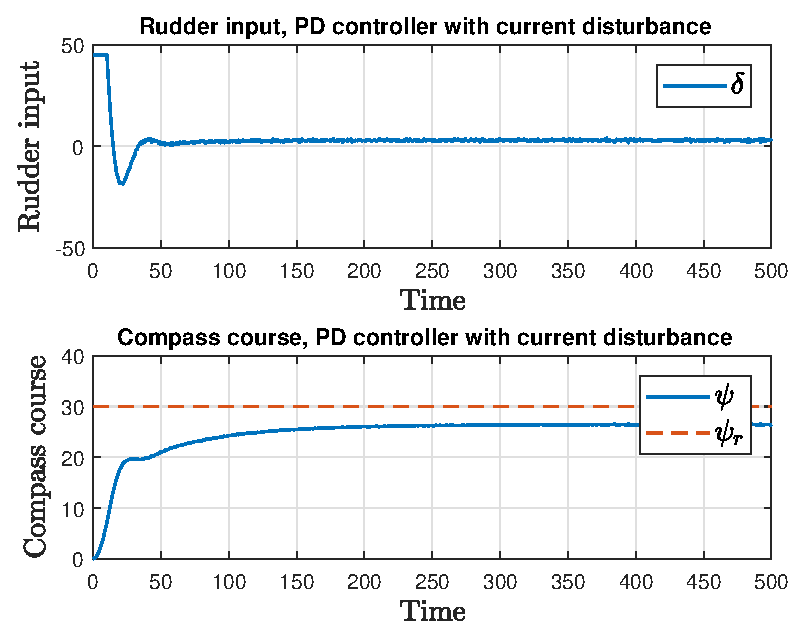
\includegraphics[width = 1.00\textwidth]{figures/plots/P5p3c_rudder_heading.eps}
    \caption{Rudder input and compass course response with a PD controller. Simulated with current disturbance.}
    \label{fig:p3pc_rudder_heading}
\end{figure}
\subsection{D, Simulation with a wave disturbance}
When simulating without current disturbance but with wave disturbance the system reaches the reference of 30$\deg$. With the wave disturbance the signal has a lot of high frequency oscillations as we can see in \cref{fig:p3pd_rudder_heading}. This is due to the high frequency nature of the waves that affect the system. \\
The oscillations are quite small compared to the state and the reference. Therefore it will not affect the system too much. Moreover the noise has a mean of zero, so it will not affect the path of the ship in the long run. The actuation of the rudder is quite oscillatory. This is not ideal and would cause wear on the physical system. Later we will look at how a Kalman filter reduces the use of actuation.  
\begin{figure}
    \centering
    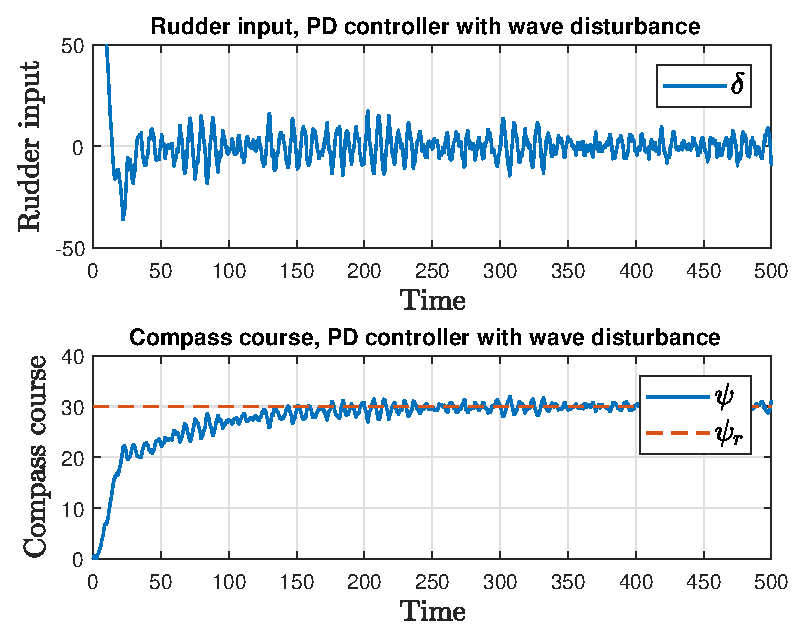
\includegraphics[width = 1.00\textwidth]{figures/plots/P5p3d_rudder_heading.eps}
    \caption{Rudder input and compass course response with a PD controller. Simlutated with wave disturbance.}
    \label{fig:p3pd_rudder_heading}
\end{figure}

\section{5.4 Observability}
\subsection{A, Creation of a state space model}
\label{seq:54a}
We want to find the system on the form $$\mathbf{\Dot{x}} = \mathbf{Ax} + \mathbf{B}u + \mathbf{Ew},  y = \mathbf{Cx} + v$$
The equations for the complete system are given in \cite{assignment} and are given by
\begin{subequations}
\begin{align}
    \dot{\xi} &= \psi_\omega\\
    \dot{\psi}_\omega &= -\omega^2_0 \xi_\omega - 2 \lambda \omega_0 \psi_\omega + K_\omega \omega_\omega\\
    \dot{\psi} &= r\\ 
    \dot{r} &= -\frac{1}{T} r + \frac{K}{T} (\delta-b)\\ 
    \dot{b} &= \omega_b\\
    y &= \psi + \psi_\omega + v.
\end{align}
\end{subequations}

Using the full model for the system we get the following
\begin{align}
\label{eq:54aModel}
    \begin{bmatrix}
        \Dot{\xi}\\
        \Dot{\psi_w}\\
        \Dot{\psi}\\
        \Dot{r}\\
        \Dot{b}
    \end{bmatrix}
    =
    \begin{bmatrix}
        0 & 1 & 0 & 0 & 0\\
        -\omega_0^2 & -2\lambda\omega_0 & 0 & 0 & 0\\
        0 & 0 & 0 & 1 & 0\\
        0 & 0 & 0 & -\frac{1}{T} & -\frac{K}{T}\\
        0 & 0 & 0 & 0 & 0
    \end{bmatrix}
    \begin{bmatrix}
        \xi_w\\
        \psi_w\\
        \psi\\
        r\\
        b
    \end{bmatrix}
    +
    \begin{bmatrix}
        0\\
        0\\
        0\\
        \frac{K}{T}\\
        0
    \end{bmatrix}
    \delta
    +
    \begin{bmatrix}
        0 & 0\\
        K_w & 0\\
        0 & 0\\
        0 & 0\\
        0 & 1
    \end{bmatrix}
    \begin{bmatrix}
        w_w\\
        w_b
    \end{bmatrix}
\end{align}
and 
\begin{align}
    y = 
    \begin{bmatrix}
        0 & 1 & 1 & 0 & 0
    \end{bmatrix}
    \begin{bmatrix}
        \xi_w\\
        \psi_w\\
        \psi\\
        r\\
        b
    \end{bmatrix}
    + v
\end{align}
Thus we can identify the matrices $\mathbf{A,B,C}$ and $\mathbf{E}$
\begin{align}\label{eq:Full_A}
    \mathbf{A} = 
    \begin{bmatrix}
        0 & 1 & 0 & 0 & 0\\
        -\omega_0^2 & -2\lambda\omega_0 & 0 & 0 & 0\\
        0 & 0 & 0 & 1 & 0\\
        0 & 0 & 0 & -\frac{1}{T} & -\frac{K}{T}\\
        0 & 0 & 0 & 0 & 0
    \end{bmatrix}
\end{align}
\begin{align}
    \mathbf{B} =
    \begin{bmatrix}
        0\\
        0\\
        0\\
        \frac{K}{T}\\
        0
    \end{bmatrix}
\end{align}
\begin{align}\label{eq:Full_C}
    \mathbf{C} = 
    \begin{bmatrix}
        0 & 1 & 1 & 0 & 0
    \end{bmatrix}
\end{align}
\begin{align}
    \mathbf{E} = 
    \begin{bmatrix}
        0 & 0\\
        K_w & 0\\
        0 & 0\\
        0 & 0\\
        0 & 1
    \end{bmatrix}
\end{align}
\subsection{B, Observability without disturbances}
A system is observable if and only if the observability matrix 
\begin{equation}
    \mathcal{O} = 
	\begin{bmatrix}
        \mathbf{C}\\
        \mathbf{CA}\\
        \vdots\\
        \mathbf{CA^{n-1}}
    \end{bmatrix}
    \label{eq:observability_matrix}
\end{equation}
has full rank\cite{Chen2014}. To check the observability we created a small MATLAB script. We check if the following statement is true \lstinline{rank(obsv(A, C)) == length(A)}. When the system has no disturbances, $\mathbf{A}$ and $\mathbf{C}$ is reduced to 
\begin{align*}
    \mathbf{A_{none}} = 
    \begin{bmatrix}
        0 & 1\\
        0 & -\frac{1}{T}
    \end{bmatrix}
    ,
    \mathbf{C_{none}} =  
    \begin{bmatrix}
        1 & 0
    \end{bmatrix}
\end{align*}
This gives us a obersvability matrix
\begin{align}
    \mathbf{\mathcal{O}_{none}} = 
    \begin{bmatrix}
        1 & 0\\
        0 & 1
    \end{bmatrix}
\end{align}
which has rank equal to the dimension of $\mathbf{A_{none}}$ and the system is thus observable.
\subsection{C, Observability with current disturbance}
With current disturbance, $\mathbf{A}$ and $\mathbf{C}$ is reduced to 
\begin{align*}
    \mathbf{A_c} = 
    \begin{bmatrix}
        0 & 1 & 0\\
        0 & -\frac{1}{T} & -\frac{K}{T}\\
        0 & 0 & 0
    \end{bmatrix}
    ,
    \mathbf{C_c} =  
    \begin{bmatrix}
        1 & 0 & 0
    \end{bmatrix}
\end{align*}
This gives us a obersvability matrix
\begin{align}
    \mathbf{\mathcal{O}_{c}} = 
    \begin{bmatrix}
        1 & 0 & 0\\
        0 & 1 & 0\\
        0 & -\frac{1}{T} & -\frac{K}{T}
    \end{bmatrix}
\end{align}
which has rank equal to the dimension of $\mathbf{A_{c}}$ and the system is thus observable.
\subsection{D, Observability with wave disturbance}
With wave disturbance, $\mathbf{A}$ and $\mathbf{C}$ is reduced to 
\begin{align*}
    \mathbf{A_w} = 
    \begin{bmatrix}
        0 & 1 & 0 & 0\\
        -\omega_0^2 & -2\lambda\omega_0 & 0 & 0\\
        0 & 0 & 0 & 1\\
        0 & 0 & 0& -\frac{1}{T}
    \end{bmatrix}
    ,
    \mathbf{C_w} =  
    \begin{bmatrix}
        0 & 1 & 1 & 0
    \end{bmatrix}
\end{align*}
This gives us a obersvability matrix
\begin{align}
    \mathbf{\mathcal{O}_w} =
    \begin{bmatrix}
        0 & 1 & 1 & 0\\
        -\omega_0^2 & -2\lambda\omega_0 & 0 & 1\\
        2\lambda\omega_0^3 & (4\lambda^2-1)\omega_0^2 & 0 & -\frac{1}{T}\\
        (4\lambda^2-1)\omega_0^4 & (4\lambda^2-1)2\lambda\omega_0^3 & 0 & \frac{1}{T^2}
    \end{bmatrix}
\end{align}
which has rank equal to the dimension of $\mathbf{A_w}$ and the system is thus observable.
\subsection{E, Observability with both disturbances}
With current and wave disturbance we use $\mathbf{A}$ and $\mathbf{C}$ given in \cref{eq:Full_A} and \cref{eq:Full_C}. This gives us a observability matrix
\begin{align}
    \mathbf{\mathcal{O}} = 
    \begin{bmatrix}
        0 & 1 & 1 & 0 & 0\\
        -\omega_0^2 & -2\lambda\omega_0 & 0 & 1 & 0\\
        2\lambda\omega_0^3 & (4\lambda^2-1)\omega_0^2 & 0 & -\frac{1}{T} & -\frac{K}{T}\\
        (4\lambda^2-1)\omega_0^4 & (4\lambda^2-1)2\lambda\omega_0^3 & 0 & \frac{1}{T^2} & \frac{K}{T^2}\\
        (2\lambda^2-1)4\lambda\omega_0^5 & (4\lambda^4-12\lambda^2+1)\omega_0^4 & 0 & -\frac{1}{T^3} & -\frac{K}{T^3}
    \end{bmatrix}
\end{align}
which has rank equal to the dimension of $\mathbf{A}$ and the system with both disturbances is thus observable.
We can conclude that the system is observable no matter the weather conditions. Especially important is the observabillity when both disturbances are present because this means that from knowledge of the output of the system we are able to determine the states \cite{Chen2014}.This enable us to use an estimator, more specifically the Kalman filter, to estimate states which we don't directly measure.  
\section{Summary}\label{sec:Summary}
 




\addcontentsline{toc}{section}{Appendix} % Remove this if you don't want the appendix included in the table of contents.
\appendix
\counterwithin{figure}{section}



% \input simply inserts the contents of the file, while \include forces a \newpage.
% See \input vs. \include: http://tex.stackexchange.com/questions/246/when-should-i-use-input-vs-include

% References
\newpage
\addcontentsline{toc}{section}{References}
\printbibliography{}
\label{sec:bibliography}

\end{document}
